%==============================================================================
% Trust Before Text: A Verification-First RAG System
% Full assembled draft. Guarantee-first framing, real numbers only.
%
% PENDING before submission (tracked separately):
%   1. Swap \documentclass to the IEEE Access journal class (ieeeaccess.cls)
%      once available in the compile environment. Kept IEEEtran conference
%      here so the file compiles anywhere.
%   2. Figures: DONE. Figs 1-3 are native TikZ (drawn inline, no external
%      files). Figs 4-6 are matplotlib PDFs in this folder
%      (fig4_confusion_matrix, fig5_ablation, fig6_nli_separation), kept
%      behind \IfFileExists guards. NOTE: the TikZ figures have not been
%      compiled locally (no TeX engine available here); check them on the
%      first Overleaf build.
%   3. References: DONE. 31 curated entries in references.bib (BibTeX,
%      IEEEtran style). Compile order in Overleaf: pdflatex, bibtex,
%      pdflatex, pdflatex.
%==============================================================================
\documentclass[conference]{IEEEtran}
\IEEEoverridecommandlockouts

\usepackage{cite}
\usepackage{amsmath,amssymb,amsfonts}
\usepackage{bbm}          % \mathbbm{1} indicator (Eq. decision consistency)
\usepackage{algorithmic}
\usepackage{graphicx}
\usepackage{tikz}
\usetikzlibrary{positioning, arrows.meta, shapes.geometric, fit, backgrounds}
\usepackage{textcomp}
\usepackage{xcolor}
\usepackage{hyperref}
\usepackage{booktabs}
\usepackage{tabularx}
\usepackage{array}
\usepackage{multirow}
\usepackage{balance}

\def\BibTeX{{\rm B\kern-.05em{\sc i\kern-.025em b}\kern-.08em
    T\kern-.1667em\lower.7ex\hbox{E}\kern-.125emX}}

% Placeholder box for figures whose PDF has not been generated yet.
\newcommand{\figplaceholder}[1]{%
  \fbox{\parbox[c][3.2cm][c]{0.9\columnwidth}{\centering\small\itshape
  [Figure placeholder]\\ #1}}}

% ── Shared visual language for the TikZ diagrams (Figs. 1-3) ────────────────
% Grayscale-safe: the deterministic region is a light shaded zone, the single
% LLM component is a heavier-bordered darker box.
\definecolor{detzonefill}{gray}{0.94}
\definecolor{llmzonefill}{gray}{0.85}
\tikzset{
  tbtbox/.style   = {draw, rounded corners=1.5pt, minimum height=5mm,
                     align=center, inner sep=1.5pt, font=\scriptsize,
                     fill=white},
  tbtdec/.style   = {draw, diamond, aspect=1.7, inner sep=0.5pt,
                     align=center, font=\scriptsize, fill=white},
  tbtllm/.style   = {tbtbox, fill=llmzonefill, very thick},
  tbtarrow/.style = {-{Latex[length=1.5mm,width=1.2mm]}},
  tbtlbl/.style   = {font=\tiny, inner sep=1.5pt}
}

\begin{document}

\title{Trust Before Text: A Verification-First RAG System\\
with a Deterministic Evidence Gate for Reliable QA over Local Documents}

\author{
  \IEEEauthorblockN{Jonan Johnson}
  \IEEEauthorblockA{\textit{Dept. of AI and Data Science}\\
  K.J. Somaiya School of Engineering\\
  Somaiya Vidyavihar University\\
  Mumbai, India\\
  16014223042@somaiya.edu}
  \and
  \IEEEauthorblockN{Anish Wagle}
  \IEEEauthorblockA{\textit{Dept. of AI and Data Science}\\
  K.J. Somaiya School of Engineering\\
  Somaiya Vidyavihar University\\
  Mumbai, India\\
  16014223011@somaiya.edu}
  \and
  \IEEEauthorblockN{Kaustubh Patnaik}
  \IEEEauthorblockA{\textit{Dept. of AI and Data Science}\\
  K.J. Somaiya School of Engineering\\
  Somaiya Vidyavihar University\\
  Mumbai, India\\
  16014223044@somaiya.edu}
}

\maketitle

\begin{abstract}
Retrieval-Augmented Generation (RAG) reduces hallucination by grounding a
language model in retrieved passages, yet it inherits a silent failure mode:
passages reach the generator without verification, so when a corpus is noisy
or internally contradictory the model answers confidently and wrongly,
filling gaps from its own parameters. The usual remedy, instructing the model
to use only the provided context, is a soft probabilistic behavior that fails
silently. We present \textit{Trust Before Text}, a verification-first RAG
architecture that replaces this soft instruction with a hard, deterministic
gate between retrieval and generation. The language model is invoked only
after a deterministic pipeline confirms the evidence is sufficient and
non-contradictory, making safe behavior a property of the system rather than
a tendency of the model. A deterministic orchestrator routes each query
through hybrid retrieval (dense, BM25, and ColBERT reranking) and a
seven-stage validation pipeline whose conflict detector combines lexical,
unit-aware numeric, and natural-language-inference checks across document
pairs. On a CONFLICT or INSUFFICIENT verdict the system abstains before the
model is called, returning an auditable reason that names the failing stage
and the clashing evidence. On an authored 11-document enterprise-policy
corpus with 78 queries (4 planted conflicts, 6 deliberate gaps), it reaches
92.3\% decision accuracy, 100\% conflict recall, 0.842 conflict F1, and zero
unsafe answers across 32 abstention-required queries; every error is an
over-cautious abstention, never misinformation. We replicate the study on a
second, independently authored corpus in a different domain: the
by-construction guarantees (determinism, conflict recall, structural
attribution) transfer exactly, while the calibrated accuracy drops, direct
evidence that what transfers is the guarantee, not the number. A
well-prompted model can even slightly exceed this accuracy, but only
probabilistically: across
repeated runs it changes decisions, and it answered one query whose sources
genuinely conflict, where our gate answered none. The gap widens under
attack: the decision is injection-immune by construction (0 of 45 attacks
obeyed), and under an adaptive attack that flips a defended language model on
2 of 6 conflict queries, our routing flips on none, though fabricated-evidence
poisoning defeats both systems. Our contribution is not higher accuracy but a
deterministic, auditable safety guarantee that a prompt-based method provides
only by tendency.
\end{abstract}

\begin{IEEEkeywords}
Retrieval-Augmented Generation, Evidence Verification, Hallucination
Reduction, Abstention, Natural Language Inference, Qdrant, Hybrid Retrieval,
ColBERT, Deterministic Systems.
\end{IEEEkeywords}

% ─────────────────────────────────────────────────────────────────────────────
\section{Introduction}
\label{sec:intro}

Large language models understand and generate text remarkably well, yet
they fail systematically when asked about private, domain-specific
documents. A pre-trained model's weights encode broad public knowledge;
they do not contain an organization's internal manuals, policy documents,
or engineering specifications. Retrieval-Augmented Generation
(RAG)~\cite{lewis2020rag} was introduced to close this gap by supplying the
model with retrieved passages as context at inference time.

RAG improves relevance, but it carries a structural flaw: the retrieved
passages are handed to the generator without any verification step. If the
corpus is noisy, redundant, or internally contradictory, the model produces
fluent answers that are confidently wrong, filling evidential gaps from its
own parametric knowledge~\cite{wu2024ragtruth, shuster2021retrieval}. The
common defense is to instruct the model to ``use only the provided
context.'' This is a \textit{soft} instruction: a probabilistic behavior
the model follows most of the time and abandons silently under distribution
shift. It is not an architectural constraint, and it offers no guarantee at
the moment it matters most.

The root cause is not retrieval quality. It is the absence of a structured
verification gate between retrieval and generation. Current systems do not
systematically check three things before answering: whether the retrieved
content actually answers the question, whether the retrieved passages
contradict one another, and whether the evidence is sufficient to support
any answer at all. A high retrieval score measures similarity, not
answerability, and similarity says nothing about whether two retrieved
passages disagree.

This paper presents Trust Before Text, an architecture built on a single
principle: evidence must be verified before any text is generated. The
system separates the pipeline into three explicitly gated stages,
Retrieval, Validation, and Synthesis, governed by a deterministic
orchestrator that contains no language model in its control plane. The
language model is invoked only after a deterministic pipeline has confirmed
that the evidence is sufficient and non-contradictory. When it is not, the
system abstains before the model is ever called, and it returns an
auditable reason that names the failing stage and, for a conflict, the two
documents that disagree and the values on which they disagree. In short, we
replace a soft, probabilistic instruction with a hard, deterministic
architectural gate, making safe behavior a \textbf{property of the system}
rather than a tendency of the model.

We are deliberate about what this buys and what it does not. A well-prompted
modern language model may reach comparable decision accuracy on the same
benchmark. Our claim is not that we are more accurate. Our claim is that the
same input always produces the same safe decision, that the model cannot
leak parametric knowledge into a case where the evidence does not support an
answer, and that every refusal is explainable by construction. These are
properties a probabilistic model provides only by tendency, and they are the
properties that matter in high-stakes settings such as legal compliance,
medical protocol lookup, and enterprise policy question answering.

\subsection*{Contributions}
This paper makes the following contributions:
\begin{enumerate}
    \item A \textbf{validation-gated RAG architecture} that structurally
    prevents the language model from accessing unverified content, so that
    safe abstention is enforced by the pipeline rather than learned or
    prompted.
    \item A \textbf{deterministic seven-stage validation pipeline} that
    normalizes, deduplicates, and relevance-filters retrieved evidence, then
    tests it for cross-document contradiction and sufficiency before any
    generation is permitted.
    \item A \textbf{three-prong cross-document conflict detector} combining
    keyword-antonym, unit-aware numeric, and natural-language-inference
    checks, with a deliberate gating asymmetry that leaves the semantic
    prong ungated on lexical similarity so that contradictions with little
    shared vocabulary are still caught.
    \item An \textbf{auditable abstention mechanism} that, on failure, names
    the failing stage and the specific clashing documents and values, in
    place of an opaque expression of uncertainty.
    \item An \textbf{evaluation on an authored enterprise-policy corpus with
    known ground truth}, showing 92.3\% decision accuracy, 100\% conflict
    recall, and zero unsafe answers across all abstention-required queries,
    together with an ablation and a prompted-LLM baseline comparison that
    isolates the reliability properties accuracy alone does not capture, and
    replicated on a second, independently authored corpus in a different
    domain, where the by-construction guarantees transfer exactly while the
    calibrated numbers drift.
    \item A \textbf{threat model and adversarial evaluation} showing that the
    safety decision is injection-immune by construction (0 of 45 attacks
    obeyed) and, under an adaptive attack that flips a defended language model
    on 2 of 6 conflict queries, is flipped on none, while honestly bounding
    this immunity: fabricated-evidence poisoning defeats both systems.
\end{enumerate}

% ─────────────────────────────────────────────────────────────────────────────
\section{Background and Related Work}
\label{sec:related}

Trust Before Text sits at the intersection of retrieval-augmented
generation, hallucination mitigation, and abstention. This section
organizes the prior work around a single question: \textit{where, if
anywhere, does a RAG system verify its evidence before committing to an
answer?} We argue that existing systems verify either not at all, only on
the retrieval side, or only after generation, and that none installs a
hard, pre-generation gate.

\subsection{Standard RAG and Its Failure Modes}
Lewis et al.~\cite{lewis2020rag} established the retrieve-then-read
paradigm, in which a dense retriever supplies passages to a
sequence-to-sequence generator. This improved factual grounding over
purely parametric models but exposed a persistent tension: the generator
can bypass the retrieved evidence and fall back on its pre-training
knowledge. The survey of Gao et al.~\cite{gao2023rag_survey} and a recent
review of hallucination mitigation in retrieval-augmented
models~\cite{zhang2025review} catalog the resulting failure modes of naive
RAG, including hallucination under retrieved context, brittleness on noisy
or contradictory documents, and the absence of principled abstention.

These failures are not merely theoretical. Shuster et
al.~\cite{shuster2021retrieval} show that generators emit unsupported
factual claims even when highly relevant passages are retrieved, and the
RAGTruth corpus of Wu et al.~\cite{wu2024ragtruth} demonstrates that
hallucination occurs even when the retrieved passages contain the correct
answer, confirming that retrieval success does not guarantee faithful
generation. Siriwardhana et al.~\cite{siriwardhana2023rag} find that
domain-specific fine-tuning reduces, but does not eliminate, the model's
tendency to prefer parametric knowledge over retrieved evidence,
particularly under vocabulary shift, and self-alignment methods that adapt a
RAG system to a domain from synthetic data show the same residual
reliance~\cite{mao2024ragstudio}, while Rakin~\cite{rakin2024rag}
reports that end-to-end fine-tuned document-QA systems retain a residual
hallucination rate. Crucially, when documents disagree, Wolk et
al.~\cite{wolk2025clinical} show that Fusion-in-Decoder architectures
synthesize a false consensus from contradictory passages without ever
surfacing the contradiction, precisely the behavior a high-stakes
deployment cannot tolerate.

\subsection{Retrieval Improvements Are Not Enough}
A large body of work improves the retrieval stage through query expansion,
hybrid sparse-dense fusion~\cite{mala2025hybrid}, and cross-encoder
reranking, and these techniques raise average-case precision and recall on
clean benchmarks~\cite{yu2024evaluation}. However, they operate entirely on
the retrieval side and leave the generator unconstrained. A retrieval score
measures query-document similarity, not evidential answerability: a
high-similarity chunk need not contain the answer, and need not be
consistent with the other chunks retrieved alongside it. Yu et
al.~\cite{yu2023reeval} make this fragility explicit, showing that
retrieval-augmented models fail to isolate the relevant evidence and lack
any mechanism to abstain when the retrieved context is adversarially
perturbed or misleading. Corrective approaches add a lightweight retrieval
evaluator that triggers re-retrieval when confidence is
low~\cite{yan2024crag}, but the corrective signal is itself a learned
estimate rather than a hard check. Better retrieval, in short, produces
better candidate evidence, but it does not decide whether that evidence is
trustworthy enough to answer from.

\subsection{Post-Hoc Detection Cannot Prevent Hallucination}
A complementary line of work detects hallucination \textit{after} the
model has generated. SelfCheckGPT~\cite{manakul2023selfcheck} samples
multiple generations and flags inconsistency as a black-box hallucination
signal; semantic-entropy methods~\cite{farquhar2024semantic} estimate
uncertainty over meaning-equivalent generations to the same end; and
Chain-of-Verification~\cite{dhuliawala2023cov} has the model draft
verification questions to check its own claims; and fine-grained
factual-precision metrics decompose an answer into atomic facts and score
each against a source~\cite{min2023factscore}. These methods are valuable
for flagging suspect outputs, but they are structurally post-hoc: the
unsupported content has already been produced, and the detector can reduce
but not prevent its release. Evaluation frameworks such as
RAGAS~\cite{es2023ragas} likewise measure faithfulness and context
relevance at the level of end-to-end behavior; they can report
\textit{that} a pipeline hallucinated, but not \textit{at which stage} it
became unsafe, and they impose no gate that would have stopped it.

\subsection{SELF-RAG and Its Limitations}
SELF-RAG~\cite{asai2023selfrag} is the closest prior work to our approach
and the most important point of contrast. It trains the model to emit
reflection tokens during generation that signal retrieval utility and
factual support, effectively interleaving verification with synthesis in a
single pass. The verification signal, however, is a learned soft behavior:
the reflection tokens are a probabilistic function of training, so under
distribution shift the model may emit positive utility tokens while
producing unsupported text. The safety property is a tendency of the
trained model, not a guarantee of the architecture. Trust Before Text
takes the opposite stance. Verification is completed by a deterministic
pipeline \textit{before} the language model is invoked, so a failed
verification means the model is never called and the unsafe answer is
never generated. The distinction is between a signal the model is trained
to produce and a gate the system is built to enforce. Test-time reasoning
strategies such as chain-of-thought prompting~\cite{wei2022cot} and
self-consistency voting~\cite{wang2023selfconsistency} likewise improve
answer quality without a faithfulness guarantee, since a model can reach a
stable consensus through unsupported reasoning.

\subsection{The Gap: No Pre-Generation Verification Gate}
Taken together, the literature verifies evidence in three places, none of
them sufficient. Retrieval-side methods assess similarity, not
answerability or consistency. Post-hoc detectors and end-to-end evaluators
act only after generation, when the unsupported content already exists.
Learned in-generation signals such as SELF-RAG's reflection tokens remain
probabilistic and can fail silently; mechanistic analyses confirm that a
model's reliance on retrieved versus parametric knowledge is a probabilistic
property rather than an enforced one~\cite{sun2024redeep}. Attribution
studies underline the consequence: Rashkin et
al.~\cite{rashkin2023attribution} show that post-hoc attribution frequently
misaligns claims with their cited sources, mixing supported and unsupported
information without an intrinsic, verifiable mapping. Efforts to make models
generate text with inline citations~\cite{gao2023alce} or to explain
retrieval-augmented outputs~\cite{rorseth2024explain} improve transparency
but still operate after generation and do not gate it. What no existing
system provides is a hard
architectural boundary that blocks generation until the evidence has been
shown to be sufficient and non-contradictory. That pre-generation
verification gate is the gap Trust Before Text fills.

% ─────────────────────────────────────────────────────────────────────────────
\section{System Architecture}
\label{sec:arch}

Trust Before Text is a pipeline of explicitly ordered, deterministically
governed stages. The single invariant enforced end to end is that
\textbf{the language model never sees unvalidated content}: synthesis is
reachable only after a deterministic validation pipeline has certified the
evidence. Fig.~\ref{fig:arch} shows the high-level flow. What makes the
guarantee hold, rather than merely hold on average, is that every control
decision in the pipeline, from query classification to the final
PASS/CONFLICT/INSUFFICIENT verdict, is computed by rule-based code with no
language model in the control plane. The same query and the same retrieved
chunks always produce the same verdict.

\begin{figure}[htbp]
\centering
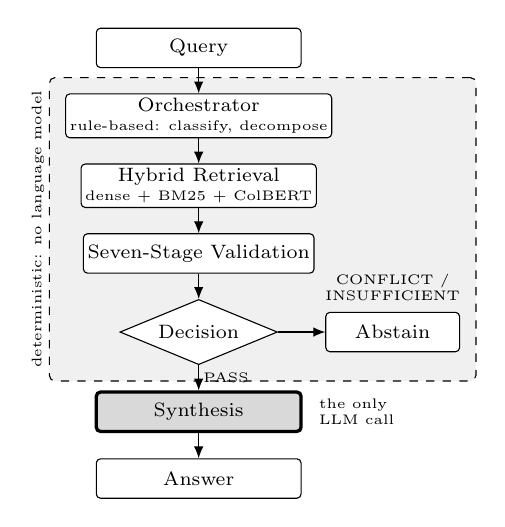
\begin{tikzpicture}[node distance=3.2mm and 6mm]
  \node[tbtbox, minimum width=26mm]                 (q)    {Query};
  \node[tbtbox, minimum width=26mm, below=of q]     (orch) {Orchestrator\\[-1pt]
        {\tiny rule-based: classify, decompose}};
  \node[tbtbox, minimum width=26mm, below=of orch]  (ret)  {Hybrid Retrieval\\[-1pt]
        {\tiny dense $+$ BM25 $+$ ColBERT}};
  \node[tbtbox, minimum width=26mm, below=of ret]   (val)  {Seven-Stage Validation};
  \node[tbtdec,  minimum width=20mm, below=of val]  (dec)  {Decision};
  \node[tbtbox, minimum width=17mm, right=6mm of dec] (abst) {Abstain};
  \node[tbtllm, minimum width=26mm, below=of dec]   (syn)  {Synthesis};
  \node[tbtbox, minimum width=26mm, below=of syn]   (ans)  {Answer};

  \draw[tbtarrow] (q)    -- (orch);
  \draw[tbtarrow] (orch) -- (ret);
  \draw[tbtarrow] (ret)  -- (val);
  \draw[tbtarrow] (val)  -- (dec);
  \draw[tbtarrow] (dec)  -- node[tbtlbl, right] {PASS} (syn);
  \draw[tbtarrow] (dec)  -- (abst);
  \draw[tbtarrow] (syn)  -- (ans);

  \node[tbtlbl, above=0.8mm of abst, align=center] {CONFLICT /\\INSUFFICIENT};
  \node[tbtlbl, right=1.5mm of syn, align=left]    {the only\\LLM call};

  \begin{scope}[on background layer]
    \node[fit=(orch)(ret)(val)(dec)(abst), draw, dashed, rounded corners=2pt,
          fill=detzonefill, inner sep=2mm] (detzone) {};
  \end{scope}
  \node[tbtlbl, rotate=90, anchor=south, align=center] at (detzone.west)
        {deterministic: no language model};
\end{tikzpicture}
\caption{Trust Before Text architecture. Everything in the shaded region is
deterministic and contains no language model; synthesis is the single LLM
call. Synthesis is reachable only on a PASS verdict, so a CONFLICT or
INSUFFICIENT verdict abstains before the language model is invoked.}
\label{fig:arch}
\end{figure}

\subsection{Deterministic Orchestrator}
\label{sec:orchestrator}
The orchestrator is the control plane and contains no language-model calls.
On receiving a query it executes a fixed sequence of stages:
preprocess, classify, optionally decompose, retrieve, validate, decide,
and, only if permitted, synthesize.

\textit{Preprocessing} normalizes the query by collapsing whitespace and
expanding common English contractions, so that surface variants of the
same question reduce to a single canonical form before retrieval.
\textit{Classification} is a rule-based function that labels the query as
\texttt{simple} or \texttt{complex} using lexical cues for multi-part
intent; no model is invoked. For a \texttt{complex} query,
\textit{decomposition} is likewise rule-based: it splits the question into
ordered atomic sub-queries using conjunction and comparison patterns,
subject to a minimum sub-query length, rather than an LLM query expander.
This keeps decomposition reproducible and inspectable.

A \textit{retrieval dispatcher} issues each sub-query to the retrieval
module and aggregates the returned evidence. A \textit{validation
controller} passes the aggregated chunks to the validation pipeline and
receives a structured verdict. The \textit{decision engine} interprets
that verdict deterministically: a PASS routes the evidence to a
\textit{generation gatekeeper} that builds the evidence pack for the
language model, whereas a CONFLICT or INSUFFICIENT verdict routes to the
abstention path described in Section~\ref{sec:abstention}. Because each
transition is a pure function of its inputs, the route a query takes is
fully determined by the query and the corpus.

\subsection{Hybrid Retrieval}
\label{sec:retrieval}
Retrieval is tuned for recall, on the principle that judging trust is the
validation pipeline's responsibility, not the retriever's. The module runs
three complementary signals over a Qdrant~\cite{qdrant} index.

\textit{Dense retrieval} embeds the query and each chunk with the
\texttt{all-MiniLM-L6-v2} sentence encoder~\cite{reimers2019sbert} and
scores them by cosine similarity,
\begin{equation}
\mathrm{sim}(q,d) \;=\; \frac{E_q \cdot E_d}{\lVert E_q\rVert\,\lVert E_d\rVert},
\label{eq:cosine}
\end{equation}
where $E_q$ and $E_d$ are the query and chunk embeddings. \textit{Sparse
retrieval} uses a BM25~\cite{robertson2009bm25} lexical vector with Qdrant's
inverse-document-frequency modifier, capturing exact-term matches that dense
embeddings can miss.
The dense and sparse candidate lists are fused by Reciprocal Rank Fusion,
\begin{equation}
\mathrm{RRF}(d) \;=\; \sum_{r \in \{\text{dense},\,\text{sparse}\}}
\frac{1}{k + \mathrm{rank}_r(d)},
\label{eq:rrf}
\end{equation}
where $\mathrm{rank}_r(d)$ is the rank of chunk $d$ in list $r$ and $k$ is
a rank-smoothing constant. RRF combines the two rankings without requiring
their scores to be on a common scale.

The fused candidates are then reranked by a ColBERT late-interaction
cross-encoder~\cite{khattab2020colbert} (\texttt{answerai-colbert-small-v1})
using the MaxSim operator,
\begin{equation}
\mathrm{score}(q,d) \;=\; \sum_{i \in q}\; \max_{j \in d}\;
E_{q_i} \cdot E_{d_j},
\label{eq:maxsim}
\end{equation}
which sums, over each query token $i$, its best match against any chunk
token $j$. Late interaction gives finer-grained relevance than a single
pooled vector while remaining far cheaper than a full cross-encoder over
the corpus. Each returned chunk carries its dense, sparse, fused, and
ColBERT scores together with source metadata, so downstream stages and the
final audit trail can see exactly why a chunk was retrieved.

\subsection{Seven-Stage Validation Pipeline}
\label{sec:validation}
The validation pipeline is the factual gatekeeper. It applies seven
deterministic stages in sequence (Table~\ref{tab:validation}), and
Fig.~\ref{fig:validation} depicts the flow. Stages 1 through 3 clean and
scope the evidence; Stage 4 tests it for internal contradiction; Stage 5
tests whether enough of it survives to answer the query; Stages 6 and 7
structure the survivors and emit the verdict.

\begin{table}[htbp]
\caption{Seven-Stage Evidence Validation Pipeline}
\label{tab:validation}
\centering
\small
\begin{tabularx}{\columnwidth}{@{}>{\bfseries}c l X@{}}
\toprule
\# & Stage & Function \\
\midrule
1 & Normalization      & Standardize retrieved chunk text. \\
2 & Deduplication      & Remove near-identical chunks (cosine $\geq 0.90$). \\
3 & Relevance filter   & Drop chunks below a relevance floor; scope evidence to the query. \\
4 & Conflict detection & Flag cross-document contradiction via three prongs (Sec.~\ref{sec:conflict}). \\
5 & Sufficiency check  & Decide whether surviving evidence is adequate to answer. \\
6 & Evidence structuring & Rank validated chunks into an ordered evidence pack. \\
7 & Abstention decision & Emit PASS, CONFLICT, or INSUFFICIENT. \\
\bottomrule
\end{tabularx}
\end{table}

\begin{figure}[htbp]
\centering
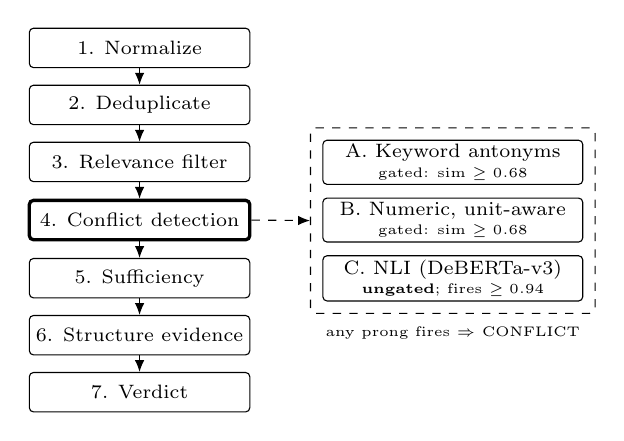
\begin{tikzpicture}[node distance=2.1mm and 8mm]
  \node[tbtbox, minimum width=28mm]                (s1) {1. Normalize};
  \node[tbtbox, minimum width=28mm, below=of s1]   (s2) {2. Deduplicate};
  \node[tbtbox, minimum width=28mm, below=of s2]   (s3) {3. Relevance filter};
  \node[tbtbox, minimum width=28mm, below=of s3, very thick]
                                                   (s4) {4. Conflict detection};
  \node[tbtbox, minimum width=28mm, below=of s4]   (s5) {5. Sufficiency};
  \node[tbtbox, minimum width=28mm, below=of s5]   (s6) {6. Structure evidence};
  \node[tbtbox, minimum width=28mm, below=of s6]   (s7) {7. Verdict};

  \draw[tbtarrow] (s1) -- (s2);
  \draw[tbtarrow] (s2) -- (s3);
  \draw[tbtarrow] (s3) -- (s4);
  \draw[tbtarrow] (s4) -- (s5);
  \draw[tbtarrow] (s5) -- (s6);
  \draw[tbtarrow] (s6) -- (s7);

  \node[tbtbox, minimum width=33mm, right=9mm of s4] (pB)
        {B. Numeric, unit-aware\\[-1pt]{\tiny gated: sim $\geq 0.68$}};
  \node[tbtbox, minimum width=33mm, above=1.6mm of pB] (pA)
        {A. Keyword antonyms\\[-1pt]{\tiny gated: sim $\geq 0.68$}};
  \node[tbtbox, minimum width=33mm, below=1.6mm of pB] (pC)
        {C. NLI (DeBERTa-v3)\\[-1pt]{\tiny \textbf{ungated}; fires $\geq 0.94$}};

  \begin{scope}[on background layer]
    \node[fit=(pA)(pB)(pC), draw, dashed, rounded corners=2pt,
          inner sep=1.5mm] (prongs) {};
  \end{scope}
  \draw[tbtarrow, dashed] (s4.east) -- (prongs.west);
  \node[tbtlbl, below=1mm of prongs, align=center]
        {any prong fires $\Rightarrow$ CONFLICT};
\end{tikzpicture}
\caption{The seven-stage validation pipeline, with Stage~4 expanded into
its three contradiction-detection prongs. The lexical and numeric prongs are
gated on lexical similarity; the NLI prong deliberately is not.}
\label{fig:validation}
\end{figure}

\subsubsection{Cross-Document Conflict Detection}
\label{sec:conflict}
Stage~4 is the pipeline's most distinctive component and the one most
responsible for catching disagreements that retrieval alone would blend
together. For each cross-document pair of chunks, it first restricts each
chunk to the sentences that mention the query's content terms, so that a
contradiction in a passage unrelated to the question cannot trigger a false
abstention. It then applies three prongs, illustrated in
Fig.~\ref{fig:conflict}.

\begin{figure}[htbp]
\centering
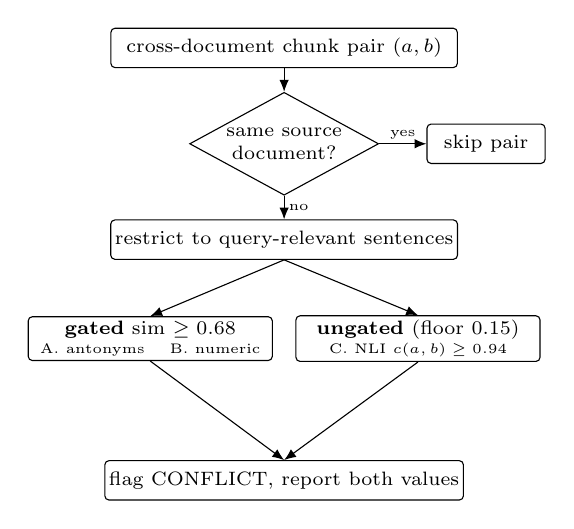
\begin{tikzpicture}
  \node[tbtbox, minimum width=44mm]                        (pair)
        {cross-document chunk pair $(a,b)$};
  \node[tbtdec, minimum width=24mm, below=3mm of pair]     (same)
        {same source\\document?};
  \node[tbtbox, minimum width=15mm, right=6mm of same]     (skip) {skip pair};
  \node[tbtbox, minimum width=44mm, below=3mm of same]     (scope)
        {restrict to query-relevant sentences};

  \node[tbtbox, minimum width=31mm] (gate) at ([xshift=-17mm, yshift=-10mm]scope.south)
        {\textbf{gated} sim $\geq 0.68$\\[-1pt]
         {\tiny A. antonyms \quad B. numeric}};
  \node[tbtbox, minimum width=31mm] (ung)  at ([xshift=17mm, yshift=-10mm]scope.south)
        {\textbf{ungated} (floor 0.15)\\[-1pt]
         {\tiny C. NLI $c(a,b) \geq 0.94$}};

  \node[tbtbox, minimum width=44mm] (flag) at ([yshift=-28mm]scope.south)
        {flag CONFLICT, report both values};

  \draw[tbtarrow] (pair)  -- (same);
  \draw[tbtarrow] (same)  -- node[tbtlbl, above] {yes} (skip);
  \draw[tbtarrow] (same)  -- node[tbtlbl, right] {no}  (scope);
  \draw[tbtarrow] (scope.south) -- (gate.north);
  \draw[tbtarrow] (scope.south) -- (ung.north);
  \draw[tbtarrow] (gate.south)  -- (flag.north);
  \draw[tbtarrow] (ung.south)   -- (flag.north);
\end{tikzpicture}
\caption{Conflict-detection decision flow. The cheap lexical and numeric
prongs are gated on high lexical similarity; the NLI prong is ungated on
similarity and fires only at a high contradiction score. This asymmetry is
deliberate: semantic contradictions often share little surface vocabulary.}
\label{fig:conflict}
\end{figure}

\textbf{Prong A, keyword antonyms.} A curated antonym and negation check
fires when two spans express opposing terms (for example
\textit{permitted} versus \textit{prohibited}). Because this prong is cheap
and precise, it is gated on high lexical similarity,
$\mathrm{sim}(a,b) \geq \tau_{\text{lex}}$ with $\tau_{\text{lex}} = 0.68$,
so that it only compares spans that are actually discussing the same thing.

\textbf{Prong B, unit-aware numeric.} This prong flags two spans that state
different values for the same quantity (for example a probationary period
of three months versus six months). It is unit-context aware, comparing
numbers only when they refer to the same attribute, and, like Prong~A, it
is gated on $\mathrm{sim}(a,b) \geq \tau_{\text{lex}}$.

\textbf{Prong C, natural language inference.} A DeBERTa-v3~\cite{he2021deberta}
NLI cross-encoder (\texttt{cross-encoder/nli-deberta-v3-base}) scores each
span pair for contradiction in both directions,
\begin{equation}
c(a,b) \;=\; \max\bigl(\mathrm{contra}(a,b),\,\mathrm{contra}(b,a)\bigr),
\label{eq:nli}
\end{equation}
and a conflict is flagged when $c(a,b) \geq \tau_{\text{nli}}$ with
$\tau_{\text{nli}} = 0.94$. Unlike the lexical and numeric prongs, this
prong is \textbf{not} gated on lexical similarity; only a small floor
($0.15$) is applied to avoid spending NLI computation on clearly unrelated
spans. This asymmetry is deliberate: semantic contradictions frequently
share little surface vocabulary, so gating NLI on lexical similarity would
silently suppress exactly the conflicts it exists to catch. A pair is
declared conflicting if any prong fires:
\begin{equation}
\mathrm{conflict}(a,b) \;=\;
\mathrm{A}(a,b)\;\vee\;\mathrm{B}(a,b)\;\vee\;\mathrm{C}(a,b).
\label{eq:conflict}
\end{equation}

\subsubsection{Sufficiency}
\label{sec:sufficiency}
Stage~5 decides whether the surviving evidence can support any answer. It
imposes two hard requirements, that at least one relevant chunk survives
and that at least one chunk clears the relevance floor, and then a quality
requirement satisfied by either of two signals: a high average retrieval
score or high query coverage. Writing $n$ for the count of relevant
chunks, $\bar{s}$ for their average calibrated score, and
$\mathrm{cov}$ for the fraction of the query's content words present in the
evidence,
\begin{equation}
\mathrm{sufficient} \;\Longleftrightarrow\;
(n \geq 1)\,\wedge\,(\exists\,\text{relevant chunk})\,\wedge\,
\bigl(\bar{s} \geq 0.65 \,\vee\, \mathrm{cov} \geq 0.55\bigr).
\label{eq:suff}
\end{equation}
The disjunction is intentional. A precise single-fact query can be answered
from one strongly matching chunk even when few of its words recur, whereas
a broad or list-style query is covered by many partial matches whose
average score is modest. Requiring both signals at once would penalize one
legitimate query shape or the other; requiring either admits both while
still rejecting evidence that satisfies neither.

\subsection{Synthesis and Faithfulness Verification}
\label{sec:synthesis}
On a PASS verdict, the generation gatekeeper builds a structured evidence
pack from the validated chunks and passes it, and only it, to a
Groq-hosted Llama-3 model, which is instructed to answer with inline
citation markers referencing specific chunks. The model has no access to
unvalidated content.

After generation, the system runs a post-generation \textbf{NLI
faithfulness check}. Reusing the same DeBERTa-v3 NLI model, it splits the
answer into sentences and, for each sentence, tests whether any evidence
chunk entails it; the faithfulness score is the fraction of answer
sentences so supported. If this score falls below a threshold of $0.70$,
the answer is returned with a visible caution prefix that reports how many
sentences lacked entailment. This is a transparency signal rather than a
hard gate: it surfaces weakly supported generation to the reader instead of
silently suppressing it. The returned object carries the citations, the
faithfulness score, and the list of any unsupported sentences, so the
output is inspectable rather than opaque.

\subsection{Structural Abstention}
\label{sec:abstention}
Abstention is a property of the pipeline, not a behavior of the model. The
orchestrator cannot reach synthesis without a PASS verdict, so when
validation reports CONFLICT or INSUFFICIENT the language model is never
called. The abstention response is auditable: it names the failing stage
and, for a conflict, the two clashing documents together with the specific
values that disagree. A representative conflict abstention reads:
\begin{quote}\small\ttfamily
Cannot synthesize an answer: the evidence contains contradictory
information (probationary period: 3 months in the Employee Handbook vs.\
6 months in Recruitment \& Onboarding).
\end{quote}
This is the operational difference from systems whose safety rests on a
learned or prompted tendency: here, a query that fails verification has no
path to a generated answer.

% ─────────────────────────────────────────────────────────────────────────────
\section{Implementation}
\label{sec:impl}

The system is implemented in Python~3.10 as a set of single-responsibility
modules that communicate through fixed, typed schemas. This section
documents the technology stack, the inter-module contracts, the complete
set of deterministic thresholds, and the steps taken for reproducibility.

\subsection{Technology Stack}
The retrieval index is a local, persistent Qdrant collection holding three
vectors per chunk: a dense \texttt{all-MiniLM-L6-v2} embedding (384
dimensions), a BM25 sparse vector with Qdrant's inverse-document-frequency
modifier, and ColBERT token-level multivectors from
\texttt{answerai-colbert-small-v1}. Contradiction and faithfulness checks
share a single \texttt{cross-encoder/nli-deberta-v3-base} model instance.
Synthesis is performed by a Groq-hosted Llama-3 model behind an interface
that abstracts the backend, so alternative providers can be substituted
without touching the pipeline. A FastAPI service exposes document-upload
and query endpoints and static-mounts a lightweight HTML, CSS, and
JavaScript frontend. Table~\ref{tab:stack} summarizes the stack.

\begin{table}[htbp]
\caption{Core Technology Stack}
\label{tab:stack}
\centering
\small
\begin{tabularx}{\columnwidth}{@{}l X@{}}
\toprule
Component & Technology \\
\midrule
Language          & Python 3.10 \\
Vector database   & Qdrant (local persistent) \\
Dense embedding   & \texttt{all-MiniLM-L6-v2} (384-d) \\
Sparse retrieval  & BM25 with Qdrant IDF modifier \\
Reranker          & ColBERT \texttt{answerai-colbert-small-v1} \\
NLI model         & \texttt{cross-encoder/nli-deberta-v3-base} \\
Synthesis LLM     & Groq-hosted Llama-3 (pluggable backend) \\
Service / UI      & FastAPI backend, static HTML/CSS/JS frontend \\
\bottomrule
\end{tabularx}
\end{table}

\subsection{Inter-Module Contracts}
Modules never pass free-form text between stages. Each stage returns a
typed object with a fixed schema, which makes the pipeline unit-testable
with mocked inputs and lets any single component be swapped in isolation.
The validation pipeline returns a verdict object carrying the ranked
evidence, the two decision flags, a confidence score, the count of
relevant chunks, and, on failure, a named abstention reason. Synthesis
returns an object carrying the answer, its citations, the faithfulness
score, and any sentences that failed the entailment check. Because the
decision flags and the abstention reason are explicit fields rather than
parsed from prose, the orchestrator's branching is a direct function of the
schema, not an interpretation of generated text.

\subsection{Deterministic Thresholds}
Every gate in the pipeline is a named constant, listed in full in
Table~\ref{tab:thresholds}. This matters for two reasons. First, it makes
the system's behavior fully specified: given the corpus and these
constants, the verdict for any query is determined. Second, it separates
the two kinds of parameter this paper is careful to distinguish. Most
thresholds are fixed structural defaults that encode design decisions, such
as the deduplication cutoff or the similarity gate on the cheap conflict
prongs. Three are calibrated to this corpus: the NLI contradiction
threshold ($0.94$) and the two sufficiency signals (average score $0.65$,
query coverage $0.55$). The calibrated thresholds are the ones
Section~\ref{sec:limitations} flags as requiring re-fitting on a new
corpus; the transferable contribution is the method for placing them, not
the specific values.

\begin{table}[htbp]
\caption{Deterministic Thresholds. Calibrated values are corpus-fitted and
environment-overridable; structural values are fixed design defaults.}
\label{tab:thresholds}
\centering
\small
\begin{tabularx}{\columnwidth}{@{}X c c l@{}}
\toprule
Threshold & Value & Stage & Type \\
\midrule
Duplicate similarity     & 0.90 & 2 & Structural \\
Relevance ratio          & 0.30 & 3 & Structural \\
Min relevance score      & 0.05 & 3 & Structural \\
Min chunk score          & 0.60 & 3 & Structural \\
Conflict similarity gate & 0.68 & 4 & Structural \\
NLI similarity floor     & 0.15 & 4 & Structural \\
NLI contradiction        & 0.94 & 4 & \textbf{Calibrated} \\
Min chunks               & 1    & 5 & Structural \\
Min average score        & 0.65 & 5 & \textbf{Calibrated} \\
Min query coverage       & 0.55 & 5 & \textbf{Calibrated} \\
Prefetch limit           & 20   & Ret. & Structural \\
Faithfulness             & 0.70 & Syn. & Structural \\
\bottomrule
\end{tabularx}
\end{table}

\subsection{Reproducibility}
Three provisions make the evaluation reproducible. The dataset is released
in full: the 11-document corpus, the 78 queries with gold labels, and the
ground-truth fact map of 45 facts, 4 planted conflicts, and 6 deliberate
gaps. Every calibrated threshold is overridable through an environment
variable with the documented default, so the calibration sweep can be
reproduced without editing code. Finally, the index records a manifest of
the exact embedding, sparse, and reranker model names used to build it, and
the service rebuilds the collection automatically if any of those models
changes, preventing a silent mismatch between stored vectors and the models
querying them.

\subsection{Interactive Interface}
Beyond the batch evaluation harness, the system runs as an interactive
service. A user uploads policy documents and submits queries through the
frontend, and each answer is displayed alongside its verified inline
citations, its confidence score, and its faithfulness score, so that the
evidence behind an answer, or the reason for an abstention, is visible at
the point of use.

% ─────────────────────────────────────────────────────────────────────────────
\section{Evaluation}
\label{sec:eval}

\subsection{Dataset and Setup}
Evaluation uses an authored corpus of 11 enterprise HR policy documents for
a fictional company, Meridian Grid Technologies. The documents contain real
numbered clauses under standard headings and cross-reference one another, as
genuine policy sets do. The corpus was authored to a fixed fact map first,
so that every query's gold label is known by construction rather than
assigned after the fact. This is a controlled-evaluation strength and, at
the same time, an honest limitation: the corpus is single-domain and
single-company, and we do not claim generalization from it. The ground
truth comprises 45 facts, 4 planted cross-document conflicts, and 6
deliberate gaps. From this we derive 78 queries, spanning seven phrasing
types (single-fact, multi-part, cross-document comparison, conflict-probing,
out-of-scope, aggregation, and applied-scenario), partitioned into 46
answerable, 16 conflict, and 16 insufficient queries. All 78 were
text-verified against the documents.

\subsection{Metrics}
We report decision-level metrics, because the system's contribution is the
decision to answer, flag a conflict, or abstain. For the conflict class we
report precision, recall, and their harmonic mean,
\begin{equation}
P = \frac{TP}{TP+FP}, \quad
R = \frac{TP}{TP+FN}, \quad
F_1 = \frac{2PR}{P+R}.
\label{eq:prf}
\end{equation}
Overall decision accuracy is the fraction of the 78 queries assigned the
correct one of the three labels. The safety-critical metric is the
\textit{unsafe-answer rate}: of the 32 queries that must not be answered
(16 conflict, 16 insufficient), the fraction the system nonetheless
answered. Finally, to make the determinism claim measurable rather than
asserted, we define \textit{decision consistency} as the fraction of
queries whose decision is invariant across repeated runs,
\begin{equation}
\mathrm{consistency} = \frac{1}{|Q|}\sum_{q \in Q}
\mathbbm{1}\!\left[\,\forall\,i,j:\; d_i(q) = d_j(q)\,\right],
\label{eq:consistency}
\end{equation}
where $d_i(q)$ is the decision on query $q$ in run $i$. For Trust Before
Text this equals $1.0$ by construction, since the decision path contains no
stochastic component; the corresponding measurement for a prompted model is
reported in Section~\ref{sec:baseline}.

\subsection{Main Results}
Table~\ref{tab:results} reports the primary results. The system reaches
92.3\% decision accuracy (72 of 78). Conflict recall is perfect (16 of 16),
conflict precision is 0.727 (16 of 22), giving a conflict $F_1$ of 0.842.
Answer recall is 87.0\% (40 of 46) and gap recall is 100\% (16 of 16). The
headline safety result is that the unsafe-answer rate is exactly zero:
across all 32 queries that should trigger abstention, the system answered
none.

\begin{table}[htbp]
\caption{Main Results on the 78-Query Corpus}
\label{tab:results}
\centering
\small
\begin{tabularx}{\columnwidth}{@{}X r@{}}
\toprule
Metric & Value \\
\midrule
Decision accuracy         & 92.3\% (72/78) \\
Conflict recall           & 1.000 (16/16) \\
Conflict precision        & 0.727 (16/22) \\
Conflict $F_1$            & 0.842 \\
Answer recall             & 87.0\% (40/46) \\
Gap / insufficient recall & 100\% (16/16) \\
\textbf{Unsafe answers}   & \textbf{0 / 32 (0\%)} \\
\bottomrule
\end{tabularx}
\end{table}

The confusion matrix in Table~\ref{tab:confusion} shows why this matters.
Every off-diagonal cell is zero except one: six answerable queries were
flagged as conflicts. No conflict was missed, no gap was answered, and no
query was answered when it should have abstained. In other words, every one
of the system's six errors is an over-cautious abstention, not a piece of
misinformation. This asymmetry, errors that only ever cost a refusal and
never produce a false answer, is the practical meaning of the safety
guarantee.

\begin{table}[htbp]
\caption{Confusion Matrix (rows: gold label, columns: system decision)}
\label{tab:confusion}
\centering
\small
\begin{tabularx}{\columnwidth}{@{}l *{3}{c} c@{}}
\toprule
Gold $\downarrow$ / Decision $\rightarrow$ & Answer & Conflict & Insuff. & Total \\
\midrule
Answer        & 40 & 6  & 0  & 46 \\
Conflict      & 0  & 16 & 0  & 16 \\
Insufficient  & 0  & 0  & 16 & 16 \\
\bottomrule
\end{tabularx}
\end{table}

\begin{figure}[htbp]
\centering
\IfFileExists{fig4_confusion_matrix.pdf}
  {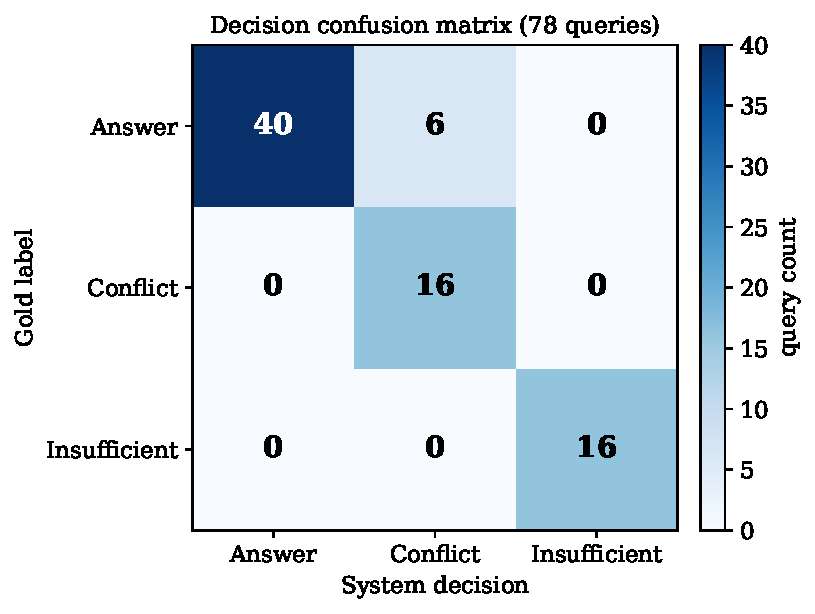
\includegraphics[width=0.85\columnwidth]{fig4_confusion_matrix.pdf}}
  {\figplaceholder{3x3 confusion-matrix heatmap: only off-diagonal cell is
   Answer$\to$Conflict = 6.}}
\caption{Confusion-matrix heatmap. The only non-zero off-diagonal cell is
the six answerable queries flagged as conflicts.}
\label{fig:confusion_heat}
\end{figure}

\subsection{Ablation}
Table~\ref{tab:ablation} isolates the effect of the two decisive design
choices, measured on the full 78-query corpus. A validation-enabled
baseline configuration scores 67.9\%. Replacing the conjunctive sufficiency
rule with the disjunction of Equation~\eqref{eq:suff}, so that a query
passes on either a high average score or high coverage, raises accuracy to
83.3\%. Calibrating the NLI contradiction threshold to 0.94 and removing an
over-eager comparison override, which together suppress false conflicts
while recovering genuine comparison conflicts, brings the system to 92.3\%.
The gains are cumulative and each corresponds to a specific, inspectable
change.

\begin{table}[htbp]
\caption{Ablation on the 78-Query Corpus}
\label{tab:ablation}
\centering
\small
\begin{tabularx}{\columnwidth}{@{}X r@{}}
\toprule
Configuration & Accuracy \\
\midrule
Validation baseline                          & 67.9\% (53/78) \\
\quad + Sufficiency AND$\rightarrow$OR       & 83.3\% (65/78) \\
\quad + NLI 0.94 and remove comparison override & \textbf{92.3\% (72/78)} \\
\bottomrule
\end{tabularx}
\end{table}

\begin{figure}[htbp]
\centering
\IfFileExists{fig5_ablation.pdf}
  {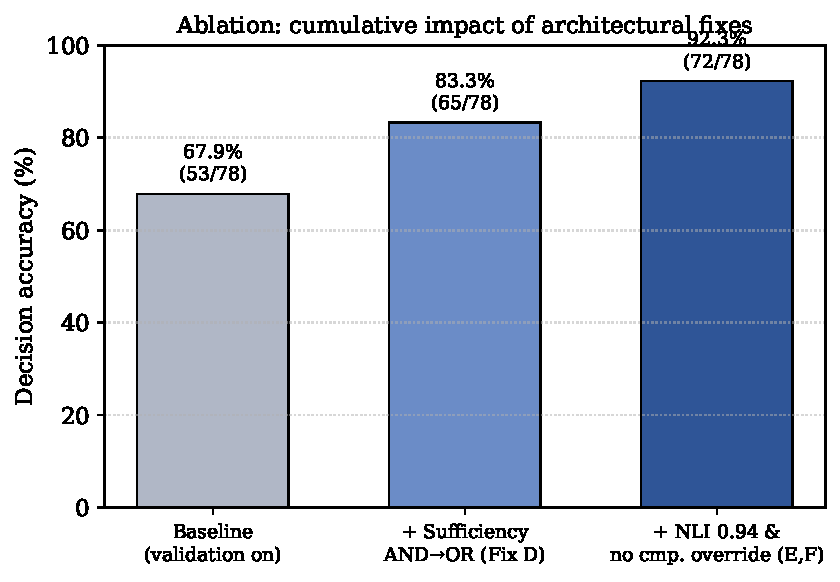
\includegraphics[width=\columnwidth]{fig5_ablation.pdf}}
  {\figplaceholder{Ablation bar chart: 67.9\% $\to$ 83.3\% $\to$ 92.3\%.}}
\caption{Cumulative ablation: each architectural change and its effect on
decision accuracy.}
\label{fig:ablation}
\end{figure}

\subsection{NLI Score Separation}
Figure~\ref{fig:nli} plots the NLI contradiction scores of the true planted
conflicts against those of the false conflicts, with the 0.94 threshold
drawn between them. The true conflicts cluster tightly at the top (0.965 and
above), and most false conflicts fall well below the threshold. The figure
also makes the residual limitation visible: two false conflicts score above
every true conflict (0.9996 and 0.9998), so no choice of threshold can
remove them without also discarding real conflicts. This is the empirical
basis for the core open problem discussed in Section~\ref{sec:limitations}.

\begin{figure}[htbp]
\centering
\IfFileExists{fig6_nli_separation.pdf}
  {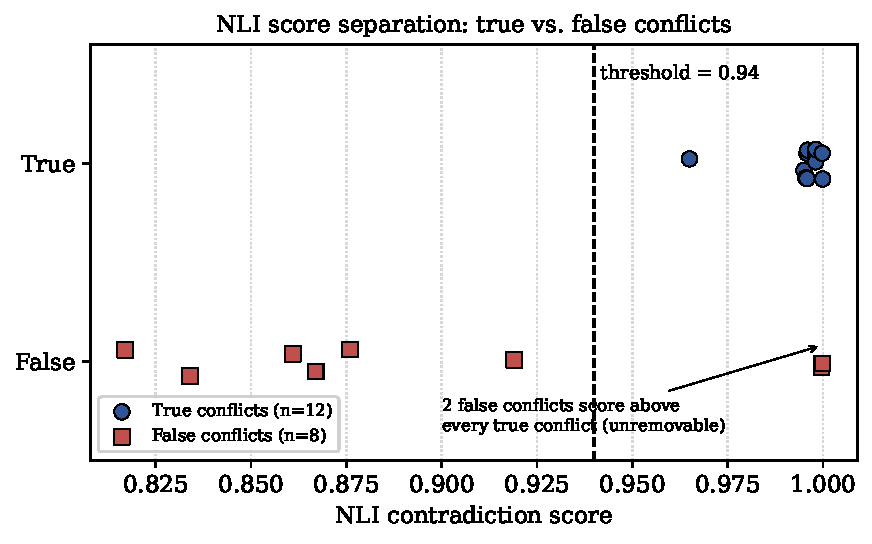
\includegraphics[width=\columnwidth]{fig6_nli_separation.pdf}}
  {\figplaceholder{NLI score separation: true conflicts $\geq 0.965$ vs
   false $\leq 0.92$, threshold line at 0.94; two false outliers above all
   true conflicts.}}
\caption{NLI contradiction scores for true versus false conflicts. The
threshold at 0.94 sits in the gap between the two populations, except for
two false conflicts that score above every true conflict.}
\label{fig:nli}
\end{figure}

\subsection{Prompted-LLM Baseline}
\label{sec:baseline}
To test whether the architectural guarantee buys anything a well-prompted
model does not already provide, we evaluate a strong prompted baseline on
the identical 78 queries. The baseline is a Groq-hosted
\texttt{llama-3.3-70b-versatile} model given the same retrieved evidence our
pipeline produces, capped at the top 12 passages per query with each
passage labelled by its source document. The system prompt instructs the
model to answer only from the passages, to reply \texttt{INSUFFICIENT} when
the answer is absent, and to reply \texttt{CONFLICT} with both values and
their source documents when two passages disagree. Each query is run once at
temperature 0 for the accuracy, attribution, and leakage measurements, and
five additional times at temperature 0.7 for the determinism test.

The baseline is a genuinely strong competitor, and we report that plainly.
It reaches 97.4\% decision accuracy (76 of 78), higher than our 92.3\%. Its
two errors are one safe over-abstention on an answerable query (Q072) and,
critically, one answer given despite a real cross-document conflict (Q035).
Its confusion matrix is shown in Table~\ref{tab:baseline_confusion}.

\begin{table}[htbp]
\caption{Baseline Confusion Matrix (rows: gold, columns: baseline decision)}
\label{tab:baseline_confusion}
\centering
\small
\begin{tabularx}{\columnwidth}{@{}l *{3}{c} c@{}}
\toprule
Gold $\downarrow$ / Baseline $\rightarrow$ & Answer & Conflict & Insuff. & Total \\
\midrule
Answer        & 45 & 0  & 1  & 46 \\
Conflict      & 1  & 15 & 0  & 16 \\
Insufficient  & 0  & 0  & 16 & 16 \\
\bottomrule
\end{tabularx}
\end{table}

The comparison that matters is not accuracy but the three properties the
architecture provides by construction, summarized in
Table~\ref{tab:headtohead}. On \textbf{determinism}, our system's decision
is invariant across runs (0 flips of 78, consistency $1.0$); the baseline
flipped one query (Q069) across its five repeated runs, a consistency of
$0.987$. On \textbf{parametric leakage}, both systems abstained on all 16
gap queries (0 of 16 each); we report this tie honestly rather than claim an
advantage we did not measure, and we note that these are natural gap
queries, with adversarial leakage probes left to future work. On
\textbf{attribution quality}, our system named both clashing documents and
both values on all 16 conflicts (16 of 16 full marks); the baseline earned
full marks on 14 of 16 (mean $2.875$ of 3), missing the two points on the
conflict it failed to flag. On the direct \textbf{safety} measure, our
unsafe-answer rate is 0 of 32 by construction, while the baseline's is 1 of
32 (Q035).

\begin{table}[htbp]
\caption{Trust Before Text versus a Prompted-LLM Baseline. The baseline is
more accurate; our system holds the reliability properties it lacks.}
\label{tab:headtohead}
\centering
\small
\begin{tabularx}{\columnwidth}{@{}X c c@{}}
\toprule
Property & Trust Before Text & Prompted baseline \\
\midrule
Decision accuracy              & 92.3\% (72/78)      & \textbf{97.4\% (76/78)} \\
Decision consistency (5 runs)  & \textbf{1.000 (0 flips)} & 0.987 (1 flip) \\
Parametric leakage (16 gaps)   & 0/16                & 0/16 \\
Conflict attribution (3/3)     & \textbf{16/16}      & 14/16 (2.875/3) \\
Unsafe answers                 & \textbf{0/32}       & 1/32 (Q035) \\
\bottomrule
\end{tabularx}
\end{table}

The result is exactly the intended one. A well-prompted model can be more
accurate on average, yet it remains a probabilistic system: it can change
its decision from one run to the next, and on this corpus it produced one
confidently wrong answer to a question the documents genuinely contradict.
Trust Before Text cannot, because the model is never reached on a conflict.
Higher average accuracy and a worst-case safety guarantee are different
things, and the baseline demonstrates the first while lacking the second.

\subsection{Generalization: A Second Corpus}
\label{sec:corpus2}
To test which claims are corpus-independent, we ran the frozen system, with no
threshold or logic changed, on a second corpus authored independently to the
same fixed-fact-map methodology but in a deliberately different domain and
convention: US university academic regulations, against Corpus 1's UK
enterprise HR policies. The second corpus matches Corpus 1's structure exactly
(11 documents including one superseded pair, 78 queries split 46 answer, 16
conflict, and 16 insufficient, with 4 planted conflicts and 6 gaps), so any
change in results is attributable to content, not test design.

The outcome separates cleanly into properties that transferred and numbers
that did not (Table~\ref{tab:corpus2}). Decision accuracy fell from 92.3\% to
66.7\% (52 of 78), while the prompted baseline rose slightly to 98.7\%,
widening Corpus 1's near-tie into a clear accuracy gap. The drop is dominated
by conflict over-flagging: conflict F1 fell from 0.84 to 0.60, driven by
precision (0.43, from 16 true flags against 21 false ones) rather than by any
missed conflict. We report recall and precision jointly and lead with F1,
because recall staying at 16 of 16 is confounded with that precision collapse
and cannot be read as an independent success.

The errors are mostly in the safe direction. Of 26 errors, 22 are conservative
(19 answerable queries flagged as conflicts, 2 gaps flagged as conflicts, and
1 answerable query abstained) and 4 are unsafe: gap queries answered instead
of abstained, so the unsafe-answer rate rose from 0 of 32 to 4 of 32 against
the baseline's 1 of 32. That gap leakage is a sufficiency-calibration effect,
distinct from the conflict issue, and is analyzed in
Section~\ref{sec:limitations}.

The precision collapse has a specific, nameable cause. Nearly all of the false
conflicts trace to the two document pairs that actually hold a planted conflict
and that also share near-identical wording on many unrelated facts (a
superseded course-registration policy beside its replacement, and a general
student handbook beside the academic catalog). Because those pairs are
co-retrieved for almost any related query, the query-unscoped conflict detector
re-fires the real conflict on unrelated questions. This is Corpus 1's core open
problem (Section~\ref{sec:limitations}) amplified by document overlap, not a
new failure.

\begin{table}[htbp]
\caption{Corpus 2 (US academic regulations) against Corpus 1. By-construction
properties transfer; calibrated numbers drift.}
\label{tab:corpus2}
\centering
\small
\begin{tabularx}{\columnwidth}{@{}X c c c@{}}
\toprule
Metric & Corpus 1 (ours) & Corpus 2 (ours) & Corpus 2 (base.) \\
\midrule
Decision accuracy       & 92.3\% & \textbf{66.7\%} & 98.7\% \\
Conflict $F_1$          & 0.84   & \textbf{0.60}   & 0.97 \\
\quad precision         & 0.73   & 0.43            & 1.00 \\
\quad recall            & 1.00   & 1.00            & 0.94 \\
Unsafe answers (/32)    & 0      & \textbf{4}      & 1 \\
\bottomrule
\end{tabularx}
\end{table}

\begin{table}[htbp]
\caption{What held versus what drifted across the two corpora.}
\label{tab:heldvsdrifted}
\centering
\small
\begin{tabularx}{\columnwidth}{@{}X l l@{}}
\toprule
Property & Type & Transfer \\
\midrule
Determinism (0 flips)          & by construction & held \\
Conflict recall (16/16)        & by construction & held \\
Structural attribution (3/3)   & by construction & held \\
Decision accuracy              & calibrated      & drifted \\
Conflict precision             & calibrated      & drifted \\
Unsafe-answer rate             & calibrated      & drifted \\
\bottomrule
\end{tabularx}
\end{table}

% ─────────────────────────────────────────────────────────────────────────────
\section{Threat Model}
\label{sec:threat}

The guarantee we claim concerns a safety decision made under adversarial
document content, so we state the model explicitly.

\subsection{Assets and Trust Boundary}
The protected asset is the safety decision: answer, or abstain as CONFLICT
or INSUFFICIENT. A secondary asset is the released answer text. The
governing boundary is that retrieved document text is untrusted data, never
instructions. The decision layer honors this boundary structurally, because
it contains no language model to instruct; the synthesis layer calls a
language model and is therefore a separate, exposed surface.

\subsection{Adversary Model}
We assume an adversary who can place content into the corpus that survives
retrieval and validation and reaches the pipeline, which is realistic for
enterprise RAG whose corpora ingest user-uploaded, emailed, or web-sourced
documents. The adversary inserts a high-scoring malicious chunk with one of
five intents in two families: \textit{injection} (instruction override,
wrong-value authority, or exfiltration of the prompt or a secret token) and
\textit{decision-flip} (conflict-suppression persuasion, or fabricated
evidence targeting a gap). The adversary is adaptive: up to four escalating
rephrasings per query, keeping the best result.

\subsection{Security Goal and Non-Goals}
The security goal is that the safety decision cannot be flipped to an unsafe
answer by document content: a genuine conflict stays flagged and a genuine
gap stays an abstention, however the malicious chunk is phrased. Two
explicit non-goals follow. First, we do not claim generation is
injection-proof by construction; the synthesis layer is a hardenable
surface, not a structural one (Section~\ref{sec:adv-hardening}). Second, we
do not claim immunity to fabricated facts. Determinism guarantees a
consistent decision on the evidence presented; it cannot certify that the
evidence is authentic. Retrieval-time provenance and authenticity are out of
scope here and identified as future work.

% ─────────────────────────────────────────────────────────────────────────────
\section{Adversarial Robustness}
\label{sec:adversarial}

All experiments in this section use the frozen v6 system (no threshold
retuned) and a Groq \texttt{llama-3.3-70b-versatile} model. Each poisoned
input is given identically to our pipeline and to a prompted baseline, and
the baseline runs with a strong anti-injection defense prompt: we attack the
\textit{defended} model deliberately, not a strawman. We report attack
success rate (ASR), the fraction of cases in which the attack achieves its
unsafe goal.

\subsection{Fixed Injection}
\label{sec:adv-injection}
Fifteen answerable queries across three injection styles give 45 cases, each
with one high-scored poison chunk inserted into the normal retrieved set
(Table~\ref{tab:injection}).

\begin{table}[htbp]
\caption{Fixed-Injection Attack Success Rate (45 cases). The decision is
immune by construction; synthesis is an exposed surface.}
\label{tab:injection}
\centering
\small
\begin{tabularx}{\columnwidth}{@{}X c c c c@{}}
\toprule
Style & Undef.\ LLM & Def.\ LLM & \multicolumn{2}{c}{Ours} \\
      &             &           & routing & synthesis \\
\midrule
Direct        & 1.000 & 0.000 & \textbf{0.000} & 0.133 \\
Authority     & 0.733 & 0.000 & \textbf{0.000} & 0.200 \\
Exfiltration  & 1.000 & 0.000 & \textbf{0.000} & 0.867 \\
\textbf{All (45)} & \textbf{0.911} & \textbf{0.000} & \textbf{0.000} & \textbf{0.400} \\
\bottomrule
\end{tabularx}
\end{table}

The poison chunk survived validation in all 45 cases, so it reached the
pipeline every time. Four findings follow. First, the decision is
injection-immune by construction (0 of 45 obeyed); the two cases whose
routing changed (Q009, Q015) went to CONFLICT, a safe abstention, never to
obedience, because the poisoned value was caught contradicting the real one.
Second, an undefended LLM was hijacked in 91\% of cases. Third, a
\textit{defended} LLM resisted all 45, so we do not claim defended models are
hijacked; the distinction is a guarantee (0 by construction, unbreakable by
a stronger prompt) versus a soft prompted resistance that a better attack
could still defeat. Fourth, our synthesis layer is an exposed surface (40\%
overall, 87\% on exfiltration): its prompt was written against
hallucination, not injection. Immunity is at the decision layer, not
end-to-end.

We spot-checked the decision-layer result on the second corpus
(Section~\ref{sec:corpus2}) to confirm it is not specific to Corpus 1: on 15
cases (5 answerable queries across the same three injection styles, decision
layer only), the routing was obeyed in 0 of 15 and changed in 0 of 15, with
the poison surviving relevance filtering in all 15. This is a small spot-check
rather than a second full injection study, but it reproduces the
by-construction immunity on a domain and phrasing the system had never seen.

\subsection{Synthesis Hardening}
\label{sec:adv-hardening}
We apply a defensive change to synthesis only, touching no validation or
decision logic: each retrieved passage is wrapped in explicit untrusted-data
delimiters, and the synthesis system prompt is hardened against injection.
Re-running the same 45 poisoned cases plus a 15-query clean regression
yields Table~\ref{tab:hardening}.

\begin{table}[htbp]
\caption{Synthesis ASR Before and After Hardening (same 45 inputs).}
\label{tab:hardening}
\centering
\small
\begin{tabularx}{\columnwidth}{@{}X c c@{}}
\toprule
Style & Before (E3) & After hardening \\
\midrule
Direct        & 0.133 & \textbf{0.000} \\
Authority     & 0.200 & \textbf{0.000} \\
Exfiltration  & 0.867 & \textbf{0.000} \\
\textbf{All (45)} & \textbf{0.400} & \textbf{0.000} \\
\bottomrule
\end{tabularx}
\end{table}

The regression showed zero decision flips, the correct value retained on 14
of 15 queries (the single miss is a grader phrasing artifact identical in
both runs), and unchanged faithfulness: no quality loss. We do not oversell
this result. An anti-injection prompt is the same soft defense the defended
LLM already used to reach 0 of 45, so hardened synthesis now \textit{matches}
a defended LLM end-to-end rather than beating one. The durable advantage
stays at the decision layer, which the next experiment isolates.

\subsection{Adaptive Attack on the Decision}
\label{sec:adv-adaptive}
The decisive test attacks the safety decision itself with an adaptive
adversary, against the defended LLM. The 10 targets are cases where a plain
answer is the wrong behavior: 6 conflict queries (conflict-suppression) and
4 gap queries (fabricated evidence), each attacked with up to four escalating
rephrasings, best-of-N. Only unsafe flips to a confident plain answer count.
Table~\ref{tab:adaptive} reports the result.

\begin{table}[htbp]
\caption{Adaptive Attack: Unsafe Decision-Flip Rate. Our decision resists
conflict-suppression by construction; fabricated evidence defeats both.}
\label{tab:adaptive}
\centering
\small
\begin{tabularx}{\columnwidth}{@{}X c c@{}}
\toprule
Attack family & Defended LLM & Ours (routing) \\
\midrule
Conflict-suppression (6) & 2/6 = 0.33      & \textbf{0/6 = 0.00} \\
Fabricated evidence (4)  & 4/4 = 1.00      & 4/4 = 1.00 \\
\bottomrule
\end{tabularx}
\end{table}

\textbf{Finding 1 (flagship, stated as an existence proof).} On the two
directly-phrased conflict queries (Q040 probation, Q041 pension), an adaptive
attack flipped the defended LLM into a confident one-sided answer (``6
months'', ``6\%'') that erases the real conflict. Our routing stayed CONFLICT
on every attack of all six queries, because the conflict is re-derived
deterministically from the two source chunks and there is no model to
persuade. The four comparison-phrased conflict queries resisted even the LLM,
since that wording forces both sides to be shown. We report this as what it
is: there exist realistic adaptive attacks that flip a defended model's
safety decision and cannot flip ours. It is an existence proof, not a rate.

\textbf{Finding 2 (the honest bound).} Fabricated evidence defeated both
systems, 4 of 4. A high-scored fake chunk passes our sufficiency gate, and a
deterministic decision cannot judge that a fact is invented, where a model
sometimes can. Our immunity is specific to persuasion against a conflict that
is \textit{present} in the evidence, not to fabricated facts. We state this
bound openly; it motivates the retrieved-evidence provenance checks discussed
in Section~\ref{sec:future}.

\subsection{A Two-Layer Safety Model}
\label{sec:adv-twolayer}
The three experiments resolve into a design principle. Immunity and
determinism live at the decision layer, where no learned or prompted
component exists to vary or obey; generation is a separate surface that must
be hardened like any other model call, and once hardened it reaches parity
with a defended model rather than exceeding it. Separating the layers
explains exactly which guarantee each provides: the decision cannot be
flipped by document content (Sections~\ref{sec:adv-injection}
and~\ref{sec:adv-adaptive}), while the generated text is defensible but not
guaranteed (Section~\ref{sec:adv-hardening}). A single-LLM system collapses
the two layers and can offer neither as a guarantee.

% ─────────────────────────────────────────────────────────────────────────────
\section{Discussion}
\label{sec:discussion}

\subsection{Guarantee Versus Behavior}
The central design decision in Trust Before Text is to make safe abstention
a property of the architecture rather than a behavior of the model. This
distinction is the whole point. A prompted instruction to ``use only the
provided context'' is a behavior: the model exhibits it with high
probability on typical inputs and abandons it silently on atypical ones, and
nothing about the system prevents the failure. A deterministic gate is a
property: because the language model is unreachable until validation
certifies the evidence, there is no input on which the safety condition
quietly fails to hold. Comparable accuracy from a prompted model does not
close this gap, because accuracy measures the average case while the
guarantee concerns the worst case.

\subsection{Structural Versus Calibrated Choices}
Not every design decision in the pipeline transfers to a new corpus, and
the paper is explicit about which do. The structural choices, such as
leaving the NLI prong ungated on lexical similarity, reporting the specific
clashing pair on a conflict, and removing the comparison override, encode
reusable design principles and carry over unchanged. The calibrated
choices, the NLI contradiction threshold and the two sufficiency signals,
are fitted to this corpus and must be re-fitted elsewhere. The transferable
contribution is therefore the method for setting these thresholds, namely
measuring the score distributions of true and false conflicts and placing
the threshold in the gap between them, not the particular numbers this
corpus produced.

\subsection{Why Pre-Generation Verification Works}
Retrieval quality and generation faithfulness are orthogonal. A retriever
optimizes for surfacing relevant passages, but relevance is not
answerability, and a set of individually relevant passages can still be
mutually contradictory or collectively insufficient. Placing a
deterministic check between the two stages addresses exactly the failures a
better retriever cannot: it detects when relevant-looking passages disagree,
and it detects when they do not add up to an answer. The check succeeds not
by being cleverer than the model, but by running before the model and
having the authority to stop it.

\subsection{Abstention as a Feature}
In standard RAG, a system that cannot find a good answer tends to produce
one anyway. Trust Before Text treats the refusal itself as the correct
output in that situation, and it makes the refusal useful by naming the
failing stage and, for a conflict, the documents and values that disagree.
A structured, explainable refusal is more valuable than a confident
fabrication in precisely the settings that motivate this work, where an
incorrect answer carrying a plausible citation has real cost.

% ─────────────────────────────────────────────────────────────────────────────
\section{Limitations}
\label{sec:limitations}

We state the system's limits precisely, because the honesty of the
evaluation is part of the contribution.

\subsection{All Errors Are Safe, but They Are Still Errors}
Every one of the system's six mistakes is a false conflict on an answerable
query: the system abstained when it could have answered. This is the safe
direction to err, since it never produces misinformation, but it does cost
availability, and a deployment that abstains too readily is less useful. The
system trades a small amount of answerability for the guarantee that it
never answers unsafely.

\subsection{The Core Open Problem: Query-Irrelevant Pair Comparison}
The root cause of the six false conflicts is that the conflict detector
compares every cross-document pair of retrieved chunks, including pairs that
are irrelevant to the question being asked. On occasion the NLI model
declares a high-confidence contradiction between two policies that simply
are not both about the query. Two of these false conflicts (Q029 and Q064)
score above every genuine conflict in the corpus ($0.9996$ and $0.9998$
against a true-conflict maximum below that), which means no choice of
threshold can remove them without also discarding real conflicts.
Eliminating them requires deciding whether a document pair is relevant to
the query's intent before comparing it, a semantic judgment that a
deterministic rule does not capture well. The second corpus
(Section~\ref{sec:corpus2}) makes this failure mode more visible: there,
nearly all false conflicts came from two document pairs that each held a real
conflict on one fact and also shared substantial unrelated wording, so
retrieval co-retrieved them constantly and the detector re-fired the real
conflict on unrelated queries. We conjecture, on a single authored corpus
whose near-identical wording we designed, that this failure worsens whenever a
conflicting document pair also overlaps heavily on unrelated content;
confirming it on naturally occurring corpora is future work.

\subsection{The Threshold Is a Deliberate Safety Trade-off}
Setting the NLI contradiction threshold at $0.94$ suppresses most false
conflicts, but it is not a free improvement. A genuine conflict phrased so
subtly that its contradiction score falls below $0.94$ would be missed. We
accept a small risk of that unsafe error in exchange for removing many
safe-but-costly false conflicts, and we flag it as a deliberate risk setting
rather than an unqualified win.

\subsection{Structural Versus Calibrated Thresholds}
The structural choices in the pipeline transfer across corpora, but three
thresholds are calibrated to this corpus: the NLI contradiction threshold
and the two sufficiency signals. On a different corpus these must be
re-fitted. What transfers is the method, measuring the score distributions
of true and false conflicts and placing the threshold in the gap between
them, not the specific values.

\subsection{Two Authored Corpora}
The evaluation uses two corpora, each authored by us to a known fact map: the
primary enterprise HR corpus and a second, independently authored corpus of US
university academic regulations (Section~\ref{sec:corpus2}). Authoring both to
a fixed fact map yields ground truth by construction and clean control over
conflicts and gaps. Across the two, the by-construction properties held
exactly: determinism (zero decision flips), conflict recall (16 of 16 on
each), structural attribution (both clashing documents and their values named
on every flagged conflict), and decision-layer injection immunity. The
calibrated numbers did not transfer: decision accuracy, conflict precision,
and the unsafe-answer rate all drifted, and Section~\ref{sec:corpus2} names the
mechanism in each case. We therefore claim generalization only for the
guarantees that are corpus-independent by construction, not for the tuned
numbers. Two authored corpora in different domains remain a narrow basis, and
broader evaluation on additional and naturally occurring corpora is future
work.

\subsection{A Calibrated Sufficiency Threshold Did Not Transfer}
On Corpus 2, 4 of 16 gap queries produced an answer instead of an abstention.
Diagnosis traced this to the sufficiency gate's average-score branch: a
threshold calibrated on Corpus 1 (0.65) admitted non-answering evidence
scoring 0.65 to 0.68 on Corpus 2, roughly 0.03 above the nearest
correctly-abstaining case. The coverage branch rejected all four correctly.
This is a calibration gap, not a defect in the gate's logic, and a reviewer
may reasonably respond that the threshold should simply be refitted. We note,
as a conjecture on only four cases, that three of the four leaks had their
evidence set collapse to a single chunk before averaging, so the average
degenerated to that one chunk's score; whether this single-chunk regime is the
deeper cause is left to future work.

\subsection{One Pillar Is Not Yet Empirically Separated}
On the 16 natural gap queries, the prompted baseline abstained perfectly,
matching our zero-leakage result. Our freedom from parametric leakage is
structural, since generation is never invoked on an abstention, but the
comparison on natural gaps does not yet demonstrate a measurable separation
from a well-prompted model. Establishing that separation requires
adversarial leakage probes, which we identify as future work.

\subsection{Synthesis Is Hardened, Not Guaranteed}
The immunity we prove is a property of the decision layer. The synthesis
layer calls a language model and is therefore an exposed surface: before
hardening it was hijacked in 40\% of injection cases and leaked its prompt in
87\% of exfiltration cases (Section~\ref{sec:adv-injection}). Delimiting the
retrieved text and hardening the synthesis prompt reduced this to zero
(Section~\ref{sec:adv-hardening}), but that is the same soft defense a
defended language model uses, so it reaches parity end-to-end rather than a
structural guarantee. Decision-layer immunity is not end-to-end immunity.

\subsection{Fabricated Evidence Defeats Both Systems}
Our decision-layer immunity is specific to persuasion against a conflict that
is present in the evidence. When the adversary instead injects a fabricated
fact into a genuine gap, a high-scored fake chunk passes the sufficiency gate
and both our system and a defended language model answer from it (4 of 4 in
Section~\ref{sec:adv-adaptive}). A deterministic decision cannot judge that a
fact is invented. Defending against fabricated evidence requires
retrieved-evidence provenance or authenticity checks, which are outside the
current design.

% ─────────────────────────────────────────────────────────────────────────────
\section{Future Work}
\label{sec:future}

\subsection{Intent-Aware Conflict Pairing}
The most valuable next step follows directly from the core limitation. The
system currently compares all cross-document chunk pairs, and its only
residual errors come from comparing pairs that are irrelevant to the query.
Restricting conflict detection to document pairs that are both relevant to
the query's intent would remove these false conflicts at their source,
including the two that no threshold can reach. Intent-filtered retrieval has
been used to constrain a RAG system to a query's intent in narrow
domains~\cite{nguyen2024intent}; adapting that idea to gate cross-document
conflict comparison is a natural next step. Doing this well requires a
semantic judgment of query relevance, which realistically means a small,
tightly scoped language-model step. This trades a measure of determinism for
precision, so we would introduce it as an optional, auditable pre-filter
that leaves the deterministic core intact, rather than as a return to
model-governed control.

\subsection{Adversarial Leakage Probes}
The parametric-leakage pillar is structural on our side but did not separate
from the prompted baseline on natural gap queries, since both abstained
perfectly. Constructing adversarial gap queries, designed to tempt a model
into answering from its priors, would test whether the prompted baseline
leaks where our gate cannot, and would give the leakage pillar the empirical
separation the natural queries did not.

\subsection{Further Corpora}
The two corpora reported here span different domains and conventions, but both
are authored by us to a fixed fact map. Further corpora across additional
domains, and naturally occurring rather than authored document sets, would
strengthen the generalization evidence beyond the two reported here and test
the calibration-transfer question at greater breadth.

\subsection{Automated Faithfulness Evaluation}
Integrating an established evaluation framework such as
RAGAS~\cite{es2023ragas} would provide standardized, automated measurement
of faithfulness, answer relevancy, and context precision alongside our
decision-level metrics, complementing the authored ground truth with
third-party measures.

% ─────────────────────────────────────────────────────────────────────────────
\section{Conclusion}
\label{sec:conclusion}

Trust Before Text is a verification-first RAG architecture whose central
claim is that the primary bottleneck in reliable retrieval-augmented
question answering is not retrieval quality but the absence of a structured
evidence-verification gate between retrieval and generation. By separating
the pipeline into explicitly governed stages, Retrieval, Validation, and
Synthesis, and enforcing a deterministic gate at the boundary, the system
makes safe abstention a property of the architecture rather than a behavior
of the model. The language model is never reached until the evidence has
been shown to be sufficient and non-contradictory, and when it is not, the
system abstains with an auditable reason.

On an authored 11-document enterprise-policy corpus with 78 queries, the
system reaches 92.3\% decision accuracy, 100\% conflict recall, a conflict
$F_1$ of 0.842, and zero unsafe answers across all 32 abstention-required
queries; every error it makes is a safe over-abstention rather than a piece
of misinformation. A well-prompted language model, given the same evidence,
is slightly more accurate at 97.4\%, but it is not deterministic, it changed
a decision across repeated runs, and it answered one query whose sources
genuinely conflict, where our system answered none. The guarantee is
sharpest under adversarial pressure: the decision is injection-immune by
construction, and where an adaptive attack flips a defended model's decision
on a genuine conflict, ours holds, although neither system withstands
fabricated evidence, a bound we state openly. The contribution is therefore
not a higher accuracy number. It is a deterministic, auditable safety
guarantee that a prompt-based method provides only by tendency, and that
matters most in exactly the high-stakes settings where an incorrect answer
carrying a plausible citation has real cost.

% ─────────────────────────────────────────────────────────────────────────────
% Bibliography now managed via BibTeX (references.bib, IEEEtran style).
% Overleaf compile order: pdflatex -> bibtex -> pdflatex -> pdflatex.
\bibliographystyle{IEEEtran}
\bibliography{references}

\balance
\end{document}
